%% bare_jrnl.tex
%% V1.4b
%% 2015/08/26
%% by Michael Shell
%% see http://www.michaelshell.org/
%% for current contact information.
%%
%% This is a skeleton file demonstrating the use of IEEEtran.cls
%% (requires IEEEtran.cls version 1.8b or later) with an IEEE
%% journal paper.
%%
%% Support sites:
%% http://www.michaelshell.org/tex/ieeetran/
%% http://www.ctan.org/pkg/ieeetran
%% and
%% http://www.ieee.org/

%%*************************************************************************
%% Legal Notice:
%% This code is offered as-is without any warranty either expressed or
%% implied; without even the implied warranty of MERCHANTABILITY or
%% FITNESS FOR A PARTICULAR PURPOSE! 
%% User assumes all risk.
%% In no event shall the IEEE or any contributor to this code be liable for
%% any damages or losses, including, but not limited to, incidental,
%% consequential, or any other damages, resulting from the use or misuse
%% of any information contained here.
%%
%% All comments are the opinions of their respective authors and are not
%% necessarily endorsed by the IEEE.
%%
%% This work is distributed under the LaTeX Project Public License (LPPL)
%% ( http://www.latex-project.org/ ) version 1.3, and may be freely used,
%% distributed and modified. A copy of the LPPL, version 1.3, is included
%% in the base LaTeX documentation of all distributions of LaTeX released
%% 2003/12/01 or later.
%% Retain all contribution notices and credits.
%% ** Modified files should be clearly indicated as such, including  **
%% ** renaming them and changing author support contact information. **
%%*************************************************************************


% *** Authors should verify (and, if needed, correct) their LaTeX system  ***
% *** with the testflow diagnostic prior to trusting their LaTeX platform ***
% *** with production work. The IEEE's font choices and paper sizes can   ***
% *** trigger bugs that do not appear when using other class files.       ***                          ***
% The testflow support page is at:
% http://www.michaelshell.org/tex/testflow/



\documentclass[journal]{IEEEtran}
%
% If IEEEtran.cls has not been installed into the LaTeX system files,
% manually specify the path to it like:
% \documentclass[journal]{../sty/IEEEtran}





% Some very useful LaTeX packages include:
% (uncomment the ones you want to load)


% *** MISC UTILITY PACKAGES ***
%
%\usepackage{ifpdf}
% Heiko Oberdiek's ifpdf.sty is very useful if you need conditional
% compilation based on whether the output is pdf or dvi.
% usage:
% \ifpdf
%   % pdf code
% \else
%   % dvi code
% \fi
% The latest version of ifpdf.sty can be obtained from:
% http://www.ctan.org/pkg/ifpdf
% Also, note that IEEEtran.cls V1.7 and later provides a builtin
% \ifCLASSINFOpdf conditional that works the same way.
% When switching from latex to pdflatex and vice-versa, the compiler may
% have to be run twice to clear warning/error messages.






% *** CITATION PACKAGES ***
%
%\usepackage{cite}
% cite.sty was written by Donald Arseneau
% V1.6 and later of IEEEtran pre-defines the format of the cite.sty package
% \cite{} output to follow that of the IEEE. Loading the cite package will
% result in citation numbers being automatically sorted and properly
% "compressed/ranged". e.g., [1], [9], [2], [7], [5], [6] without using
% cite.sty will become [1], [2], [5]--[7], [9] using cite.sty. cite.sty's
% \cite will automatically add leading space, if needed. Use cite.sty's
% noadjust option (cite.sty V3.8 and later) if you want to turn this off
% such as if a citation ever needs to be enclosed in parenthesis.
% cite.sty is already installed on most LaTeX systems. Be sure and use
% version 5.0 (2009-03-20) and later if using hyperref.sty.
% The latest version can be obtained at:
% http://www.ctan.org/pkg/cite
% The documentation is contained in the cite.sty file itself.






% *** GRAPHICS RELATED PACKAGES ***
%
\ifCLASSINFOpdf
  \usepackage[pdftex]{graphicx}
  \usepackage{subcaption}  % Periot's: for subfigures and subcaptions
  % declare the path(s) where your graphic files are
  % \graphicspath{{../pdf/}{../jpeg/}}
  % and their extensions so you won't have to specify these with
  % every instance of \includegraphics
  % \DeclareGraphicsExtensions{.pdf,.jpeg,.png}
\else
  % or other class option (dvipsone, dvipdf, if not using dvips). graphicx
  % will default to the driver specified in the system graphics.cfg if no
  % driver is specified.
  % \usepackage[dvips]{graphicx}
  % declare the path(s) where your graphic files are
  % \graphicspath{{../eps/}}
  % and their extensions so you won't have to specify these with
  % every instance of \includegraphics
  % \DeclareGraphicsExtensions{.eps}
\fi
% graphicx was written by David Carlisle and Sebastian Rahtz. It is
% required if you want graphics, photos, etc. graphicx.sty is already
% installed on most LaTeX systems. The latest version and documentation
% can be obtained at: 
% http://www.ctan.org/pkg/graphicx
% Another good source of documentation is "Using Imported Graphics in
% LaTeX2e" by Keith Reckdahl which can be found at:
% http://www.ctan.org/pkg/epslatex
%
% latex, and pdflatex in dvi mode, support graphics in encapsulated
% postscript (.eps) format. pdflatex in pdf mode supports graphics
% in .pdf, .jpeg, .png and .mps (metapost) formats. Users should ensure
% that all non-photo figures use a vector format (.eps, .pdf, .mps) and
% not a bitmapped formats (.jpeg, .png). The IEEE frowns on bitmapped formats
% which can result in "jaggedy"/blurry rendering of lines and letters as
% well as large increases in file sizes.
%
% You can find documentation about the pdfTeX application at:
% http://www.tug.org/applications/pdftex





% *** MATH PACKAGES ***
%
%\usepackage{amsmath}
% A popular package from the American Mathematical Society that provides
% many useful and powerful commands for dealing with mathematics.
%
% Note that the amsmath package sets \interdisplaylinepenalty to 10000
% thus preventing page breaks from occurring within multiline equations. Use:
%\interdisplaylinepenalty=2500
% after loading amsmath to restore such page breaks as IEEEtran.cls normally
% does. amsmath.sty is already installed on most LaTeX systems. The latest
% version and documentation can be obtained at:
% http://www.ctan.org/pkg/amsmath


 


% *** SPECIALIZED LIST PACKAGES ***
%
%\usepackage{algorithmic}
% algorithmic.sty was written by Peter Williams and Rogerio Brito.
% This package provides an algorithmic environment fo describing algorithms.
% You can use the algorithmic environment in-text or within a figure
% environment to provide for a floating algorithm. Do NOT use the algorithm
% floating environment provided by algorithm.sty (by the same authors) or
% algorithm2e.sty (by Christophe Fiorio) as the IEEE does not use dedicated
% algorithm float types and packages that provide these will not provide
% correct IEEE style captions. The latest version and documentation of
% algorithmic.sty can be obtained at:
% http://www.ctan.org/pkg/algorithms
% Also of interest may be the (relatively newer and more customizable)
% algorithmicx.sty package by Szasz Janos:
% http://www.ctan.org/pkg/algorithmicx




% *** ALIGNMENT PACKAGES ***
%
%\usepackage{array}
% Frank Mittelbach's and David Carlisle's array.sty patches and improves
% the standard LaTeX2e array and tabular environments to provide better
% appearance and additional user controls. As the default LaTeX2e table
% generation code is lacking to the point of almost being broken with
% respect to the quality of the end results, all users are strongly
% advised to use an enhanced (at the very least that provided by array.sty)
% set of table tools. array.sty is already installed on most systems. The
% latest version and documentation can be obtained at:
% http://www.ctan.org/pkg/array


% IEEEtran contains the IEEEeqnarray family of commands that can be used to
% generate multiline equations as well as matrices, tables, etc., of high
% quality.




% *** SUBFIGURE PACKAGES ***
%\ifCLASSOPTIONcompsoc
%  \usepackage[caption=false,font=normalsize,labelfont=sf,textfont=sf]{subfig}
%\else
%  \usepackage[caption=false,font=footnotesize]{subfig}
%\fi
% subfig.sty, written by Steven Douglas Cochran, is the modern replacement
% for subfigure.sty, the latter of which is no longer maintained and is
% incompatible with some LaTeX packages including fixltx2e. However,
% subfig.sty requires and automatically loads Axel Sommerfeldt's caption.sty
% which will override IEEEtran.cls' handling of captions and this will result
% in non-IEEE style figure/table captions. To prevent this problem, be sure
% and invoke subfig.sty's "caption=false" package option (available since
% subfig.sty version 1.3, 2005/06/28) as this is will preserve IEEEtran.cls
% handling of captions.
% Note that the Computer Society format requires a larger sans serif font
% than the serif footnote size font used in traditional IEEE formatting
% and thus the need to invoke different subfig.sty package options depending
% on whether compsoc mode has been enabled.
%
% The latest version and documentation of subfig.sty can be obtained at:
% http://www.ctan.org/pkg/subfig




% *** FLOAT PACKAGES ***
%
%\usepackage{fixltx2e}
% fixltx2e, the successor to the earlier fix2col.sty, was written by
% Frank Mittelbach and David Carlisle. This package corrects a few problems
% in the LaTeX2e kernel, the most notable of which is that in current
% LaTeX2e releases, the ordering of single and double column floats is not
% guaranteed to be preserved. Thus, an unpatched LaTeX2e can allow a
% single column figure to be placed prior to an earlier double column
% figure.
% Be aware that LaTeX2e kernels dated 2015 and later have fixltx2e.sty's
% corrections already built into the system in which case a warning will
% be issued if an attempt is made to load fixltx2e.sty as it is no longer
% needed.
% The latest version and documentation can be found at:
% http://www.ctan.org/pkg/fixltx2e


%\usepackage{stfloats}
% stfloats.sty was written by Sigitas Tolusis. This package gives LaTeX2e
% the ability to do double column floats at the bottom of the page as well
% as the top. (e.g., "\begin{figure*}[!b]" is not normally possible in
% LaTeX2e). It also provides a command:
%\fnbelowfloat
% to enable the placement of footnotes below bottom floats (the standard
% LaTeX2e kernel puts them above bottom floats). This is an invasive package
% which rewrites many portions of the LaTeX2e float routines. It may not work
% with other packages that modify the LaTeX2e float routines. The latest
% version and documentation can be obtained at:
% http://www.ctan.org/pkg/stfloats
% Do not use the stfloats baselinefloat ability as the IEEE does not allow
% \baselineskip to stretch. Authors submitting work to the IEEE should note
% that the IEEE rarely uses double column equations and that authors should try
% to avoid such use. Do not be tempted to use the cuted.sty or midfloat.sty
% packages (also by Sigitas Tolusis) as the IEEE does not format its papers in
% such ways.
% Do not attempt to use stfloats with fixltx2e as they are incompatible.
% Instead, use Morten Hogholm'a dblfloatfix which combines the features
% of both fixltx2e and stfloats:
%
% \usepackage{dblfloatfix}
% The latest version can be found at:
% http://www.ctan.org/pkg/dblfloatfix

\usepackage{url}
% \usepackage[section]{placeins}

%\ifCLASSOPTIONcaptionsoff
%  \usepackage[nomarkers]{endfloat}
% \let\MYoriglatexcaption\caption
% \renewcommand{\caption}[2][\relax]{\MYoriglatexcaption[#2]{#2}}
%\fi
% endfloat.sty was written by James Darrell McCauley, Jeff Goldberg and 
% Axel Sommerfeldt. This package may be useful when used in conjunction with 
% IEEEtran.cls'  captionsoff option. Some IEEE journals/societies require that
% submissions have lists of figures/tables at the end of the paper and that
% figures/tables without any captions are placed on a page by themselves at
% the end of the document. If needed, the draftcls IEEEtran class option or
% \CLASSINPUTbaselinestretch interface can be used to increase the line
% spacing as well. Be sure and use the nomarkers option of endfloat to
% prevent endfloat from "marking" where the figures would have been placed
% in the text. The two hack lines of code above are a slight modification of
% that suggested by in the endfloat docs (section 8.4.1) to ensure that
% the full captions always appear in the list of figures/tables - even if
% the user used the short optional argument of \caption[]{}.
% IEEE papers do not typically make use of \caption[]'s optional argument,
% so this should not be an issue. A similar trick can be used to disable
% captions of packages such as subfig.sty that lack options to turn off
% the subcaptions:
% For subfig.sty:
% \let\MYorigsubfloat\subfloat
% \renewcommand{\subfloat}[2][\relax]{\MYorigsubfloat[]{#2}}
% However, the above trick will not work if both optional arguments of
% the \subfloat command are used. Furthermore, there needs to be a
% description of each subfigure *somewhere* and endfloat does not add
% subfigure captions to its list of figures. Thus, the best approach is to
% avoid the use of subfigure captions (many IEEE journals avoid them anyway)
% and instead reference/explain all the subfigures within the main caption.
% The latest version of endfloat.sty and its documentation can obtained at:
% http://www.ctan.org/pkg/endfloat
%
% The IEEEtran \ifCLASSOPTIONcaptionsoff conditional can also be used
% later in the document, say, to conditionally put the References on a 
% page by themselves.




% *** PDF, URL AND HYPERLINK PACKAGES ***
%
%\usepackage{url}
% url.sty was written by Donald Arseneau. It provides better support for
% handling and breaking URLs. url.sty is already installed on most LaTeX
% systems. The latest version and documentation can be obtained at:
% http://www.ctan.org/pkg/url
% Basically, \url{my_url_here}.




% *** Do not adjust lengths that control margins, column widths, etc. ***
% *** Do not use packages that alter fonts (such as pslatex).         ***
% There should be no need to do such things with IEEEtran.cls V1.6 and later.
% (Unless specifically asked to do so by the journal or conference you plan
% to submit to, of course. )


% correct bad hyphenation here
\hyphenation{op-tical net-works semi-conduc-tor}

\usepackage{amsmath}
\usepackage{algorithm}
\usepackage{algpseudocode}
\usepackage{bm}
\begin{document}
%
% paper title
% Titles are generally capitalized except for words such as a, an, and, as,
% at, but, by, for, in, nor, of, on, or, the, to and up, which are usually
% not capitalized unless they are the first or last word of the title.
% Linebreaks \\ can be used within to get better formatting as desired.
% Do not put math or special symbols in the title.
\title{Infrastructure-free Multidimensional Scaling for drones swarm localization}
%
%
% author names and IEEE memberships
% note positions of commas and nonbreaking spaces ( ~ ) LaTeX will not break
% a structure at a ~ so this keeps an author's name from being broken across
% two lines.
% use \thanks{} to gain access to the first footnote area
% a separate \thanks must be used for each paragraph as LaTeX2e's \thanks
% was not built to handle multiple paragraphs
%

\author{Giacomo Mutti,~\IEEEmembership{233189},  \\
Pierfrancesco Oselin,~\IEEEmembership{229564},  \\
Riccardo Periotto,~\IEEEmembership{230266}
        }% <-this % stops a space



% note the % following the last \IEEEmembership and also \thanks - 
% these prevent an unwanted space from occurring between the last author name
% and the end of the author line. i.e., if you had this:
% 
% \author{....lastname \thanks{...} \thanks{...} }
%                     ^------------^------------^----Do not want these spaces!
%
% a space would be appended to the last name and could cause every name on that
% line to be shifted left slightly. This is one of those "LaTeX things". For
% instance, "\textbf{A} \textbf{B}" will typeset as "A B" not "AB". To get
% "AB" then you have to do: "\textbf{A}\textbf{B}"
% \thanks is no different in this regard, so shield the last } of each \thanks
% that ends a line with a % and do not let a space in before the next \thanks.
% Spaces after \IEEEmembership other than the last one are OK (and needed) as
% you are supposed to have spaces between the names. For what it is worth,
% this is a minor point as most people would not even notice if the said evil
% space somehow managed to creep in.


% The paper headers
%\markboth{Journal of \LaTeX\ Class Files,~Vol.~14, No.~8, August~2015}%
%{Shell \MakeLowercase{\textit{et al.}}: Bare Demo of IEEEtran.cls for IEEE Journals}
% The only time the second header will appear is for the odd numbered pages
% after the title page when using the twoside option.
% 
% *** Note that you probably will NOT want to include the author's ***
% *** name in the headers of peer review papers.                   ***
% You can use \ifCLASSOPTIONpeerreview for conditional compilation here if
% you desire.




% If you want to put a publisher's ID mark on the page you can do it like
% this:
%\IEEEpubid{0000--0000/00\$00.00~\copyright~2015 IEEE}
% Remember, if you use this you must call \IEEEpubidadjcol in the second
% column for its text to clear the IEEEpubid mark.



% use for special paper notices
%\IEEEspecialpapernotice{(Invited Paper)}




% make the title area
\maketitle

% As a general rule, do not put math, special symbols or citations
% in the abstract or keywords.
% ABSTRACT (200 words)
% The problem can be solved with trilateration and minimization, but this uses part of the information we can gather using UWB sensor on each drone
% We investigated how an algorithm using all the distances such as MDS behaves in solving the same problem, with considerations about different noises affecting the information we have (about the distances and about the position of the anchor).
% What we wanted to check was whether using MDS allows to achieve better results, given the larger amount of information adopted by the algorithm.
% The results show that MDS is better.

\begin{abstract}\label{sec:abstract_section}
This paper explores the localization of drones within various operational scenarios using the Multidimensional Scaling (MDS) algorithm and compares its performance with the conventional trilateration method. Drones' widespread applications, ranging from aerial photography to scientific research, necessitate precise localization even in challenging environments where GPS signals are unreliable. The MDS algorithm, capable of leveraging Ultra-Wideband (UWB) measurements, is investigated for its accuracy and robustness in comparison to trilateration. Through numerical and Software-in-the-loop simulations, MDS consistently outperforms trilateration across scenarios involving Gaussian-distributed noise in dynamics, measurements, and clock-time. Notably, this study pioneers swarm estimation via infrastructure-free measurements, wherein a designated anchor node collects data to drive the algorithm. Future research avenues are suggested, including extended-MDS integration and covariance estimation for enhanced Kalmann filter updates. This work contributes insights into optimal drone localization methods for diverse applications, highlighting MDS as a superior choice for precision and adaptability.

\end{abstract}


% Note that keywords are not normally used for peerreview papers.
%\begin{IEEEkeywords}
%IEEE, IEEEtran, journal, \LaTeX, paper, template.
%\end{IEEEkeywords}






% For peer review papers, you can put extra information on the cover
% page as needed:
% \ifCLASSOPTIONpeerreview
% \begin{center} \bfseries EDICS Category: 3-BBND \end{center}
% \fi
%
% For peerreview papers, this IEEEtran command inserts a page break and
% creates the second title. It will be ignored for other modes.
\IEEEpeerreviewmaketitle


% Introduction
\section{Introduction}\label{sec:introduction_section}

\IEEEPARstart{D}{rones} have witnessed escalating utilization across diverse sectors, revolutionizing industries with their aerial capabilities. From aerial photography, surveillance, search and rescue to agriculture, infrastructure inspection, and delivery services, drones are reshaping operational paradigms. Their ability to navigate challenging environments, gather real-time data and efficiently execute tasks has led to their integration in sectors such as filmmaking, disaster response, precision farming, and scientific research. As technological advancements continue, drones' versatile applications are expected to further expand, driving innovation and transforming industries on a global scale.
\par

Regardless of the application, the ability to determine the exact location of a drone is critical to achieving operational goals.
For example, precise localization boosts safe navigation, optimal data collection, and effective communication. More generally, it is possible to claim that it increases the chances of successful drone adoption.
Drones are typically localized using Global Positioning Systems (GPS), such as Global Navigation Satellite System (GNSS), which rely on satellites' signals to determine their position. In addition, sensors such as accelerometers, gyroscopes, and barometers aid navigation and stabilization. 
However, this global reference is not always available, especially as the range of applications stretches to remote and hardly reachable locations: indoor settings, urban canyons, and dense vegetation.
This poses a challenge to which the answer is still a topic of research.
\par

\subsection{Possible solutions}
In these circumstances, some techniques like visual odometry and SLAM (Simultaneous Localization and Mapping) are employed for computing the drone position and attitude. These methods enable drones to navigate autonomously, avoid obstacles, and execute tasks with precision.
An alternative approach, more suitable for a swarm of drones, is represented by Ultra-Wideband (UWB) signals. UWB technology operates by transmitting short-duration pulses with extremely low power across a wide frequency spectrum. UWB signals experience minimal interference and exhibit high immunity to multipath effects, making them ideal for precise distance measurement. This enables UWB-equipped drones to establish relative distances between themselves. 
\par

This set of relative distances represents a snapshot of the swarm configuration and can be used to compute the relative layout through various algorithms. 
Among these, trilateration plays the role of the most straightforward one. This method derives the position of the nodes considering their distances from 3 known points in the 2D case and 4 points in the 3D one (see Section~\ref{sec:theory_section} for more details). 
The problem can be solved with different techniques depending on the settings. If the measurements are not disturbed, the problem becomes an algebraic system of equations. On the other hand, if data are corrupted, Least-Square Minimization (LSM) can be used.
Although valuable, a shortcoming of the trilateration approach is that it only uses the distances between the nodes and the anchors, not taking advantage of the information contained in the distance measurements between non-anchor nodes.
\par

The Multidimensional Scaling (MDS) algorithm is a favored approach for leveraging UWB measurements in wireless network localization. MDS is a widely employed method for dimensionality reduction, which objective is to transforms multidimensional data into a lower-dimensional space while retaining essential information. While various dimensionality reduction techniques like PCA, factor analysis, and isomap exist, MDS stands out due to its user-friendly nature and versatile applicability.
\par

\subsection{Contribution}
The objective of this paper is to compare the performance of the two mentioned localization algorithms, namely trilateration through LSM and MDS, within a ROS 2\footnote{Robot Operating System v2} project. Through testing scripts that utilize these algorithms, the superior qualities of MDS become evident when contrasted with trilateration. MDS demonstrates robustness and precision, particularly in scenarios characterized by noise and measurement errors. 
The project's code can be found at the repository below \footnote{https://github.com/oselin/drone-pose-estimation}.

%%%

The rest of the paper is organized as follows. Section~\ref{sec:related_work} delves into the related work, presenting the currently employed Local Positioning System (LPS) techniques.\par

Subsequently, Section~\ref{sec:theory_section} provides a comprehensive elucidation of the mathematical principles behind both algorithms.
In Section~\ref{sec:methodology_section}, the project's structure is described, with an explanation about the algorithms execution, how it has been developed the simulation suites and the experiments that has been conducted.\par

Finally, results and conclusion collect the outcomes of the study and present a summary of what was done, mentioning some possible future directions.





%%%%%%%%% BELOW THE PREVIOUS VERSION 17/08/2023 h. 10:52
%%% \IEEEPARstart{D}{rones} have witnessed escalating utilization across diverse sectors, revolutionizing industries with their aerial capabilities. From aerial photography, surveillance, search and rescue to agriculture, infrastructure inspection, and delivery services, drones are reshaping operational paradigms. Their ability to navigate challenging environments, gather real-time data, and efficiently execute tasks has led to their integration in sectors such as filmmaking, disaster response, precision farming, and scientific research. As technological advancements continue, drones' versatile applications are anticipated to further expand, driving innovation and transforming industries on a global scale.
%%% \par
%%% The success of drone applications hinges on precise localization. It ensures safe navigation, optimal data collection, and effective communication. Despite the application, the ability to determine a drone's exact position is pivotal for achieving operational goals.
%%% Drones are typically localized using Global Positioning Systems (GPS), such as Global Navigation Satellite System (GNSS), which rely on signals from satellites to determine their position. Additionally, sensors like accelerometers, gyroscopes, and barometers aid in navigation and stabilization. However, this global reference is not always available, especially as the range of applications stretches in remote and hardly reachable locations: indoor settings, urban canyons, and dense vegetation.
%%% This poses a challenge to which the answer is still a topic of research.\par
%%% 
%%% 
%%% \subsection{Possible solutions}
%%% In these circumstances, some techniques like visual odometry and SLAM (Simultaneous Localization and Mapping) are employed for computing the drone position and attitude. These methods enable drones to navigate autonomously, avoid obstacles, and execute tasks with precision.
%%% An alternative approach, more suitable for a fleet of drones, is represented by Ultra-Wideband (UWB) signals. UWB technology operates by transmitting short-duration pulses with extremely low power across a wide frequency spectrum. UWB signals experience minimal interference and exhibit high immunity to multipath effects, making them ideal for precise distance measurement. This enables UWB-equipped drones to establish relative distances between themselves. 
%%% \par
%%% This set of relative distances, after proper manipulation, represents a snapshot of the swarm configuration. To compute the local relative configuration, different algorithms can be chosen. 
%%% Of these, the most straightforward are trilateration and Least-Squares  Minimization (LSM). The former can derive the position of nodes through geometry, while the latter is able to derive the position of drones by minimizing the difference between the measured distances and those obtained from position estimates.
%%% Although both algorithms are valuable, they only use the distances between each node and the anchors, not taking advantage of the information contained in all the other nodes distances.
%%% \par
%%% An algorithm that tries to take full advantage of the UWB measurements is Multi-Dimensional Scaling (MDS): it is one of the dimensionality reduction technique which has been used extensively in the recent past for wireless networks localization. MDS is one of the dimensionality reduction methods that converts multidimensional data into a lower dimensional space while preserving the crucial information. There are other dimensionality reduction techniques available, including principal component analysis (PCA), factor analysis, and isomap, but MDS is the most well-liked among them due to its ease of use and broad range of applications.
%%% \par
%%% 
%%% 
%%% \subsection{Contribution}
%%% 
%%% This paper aims at comparing the performances of the two localization algorithms LSM and MDS in a ROS 2\footnote{Robot Operating System v2} project. Testing scripts that rely on these tools further highlight the strengths of MDS when compared to LSM: its robustness and precision even in cases of high noise and measurement errors.\par
%%% The rest of the paper is organized in different sections. First, the related work will be analyzed in order to give a more detailed description of the field and of the currently used Local Positioning System (LPS) techniques.
%%% Next, Section \ref{sec:theory_section} is entirely dedicated at explaining how the two algorithms mathematically work. In Section \ref{sec:methodology_section}, the whole structure of the project is described; this comprehends a description of how we run the two algorithms, the simulation suits developed, and the experiments conducted.
%%% Finally results and conclusion collect the outcomes of the study and present a complete overview, followed by future work that can be.






% Related work
\section{Related Work}\label{sec:related_work}
The problem of determining the position of the nodes in a Wireless Sensor Network (WSN) has been a subject of research since the inception of these networks \cite{doherty_convex_2001, corbalan_self-localization_2023}.
Initially, the focus was on tracking sensor nodes within the network, as their data was inherently valuable only when coupled with accurate positional information. 
Over time, the convergence of WSNs with the Internet of Things (IoT) and the spread adoption of unmanned vehicles have sustained the interest in this field with application in both 2D and 3D scenarios \cite{popescu_survey_2019}.

% like Global Navigation Satellite System
While GPS have conventionally been employed to address localization challenges, its utilization is limited by factors such as the unavailability of global measurements in certain environments and high costs in terms of size, price, and energy consumption \cite{doherty_convex_2001}. 
Consequently, a trend followed in the literature to overcome these limitations has been the adoption of Local Positioning Systems (LPS).

In the field of LPS, a notable approach is utilizing radio frequency (RF) signal propagation for accurate localization. Ultra-Wideband (UWB) technology, known for its robustness against multipath errors, obstacle penetration, high accuracy, and cost-effectiveness, has garnered increasing interest \cite{santoro_uwb-based_2023, niculescu_energy-efficient_2023, queralta_uwb-based_2020}. Common techniques for RF-based localization include Received Signal Strength (RSS), Time of Arrival (ToA), Time Difference of Arrival (TDoA), and Angle of Arrival (AoA) methods. Despite the differences between these methods, the ultimate goal is to provide a measure of the physical distance between sensors.

Recent studies have explored UWB-based localization approaches, with a focus on static infrastructure utilizing fixed nodes (anchors) to locate other nodes (agents) within their range \cite{almansa_autocalibration_2020, patwari_locating_2005}. 
In 3D cases, when the distance of an agent from 4 anchors is known, various techniques have been developed to estimate node locations based on distance measurements \cite[Chapters 23-27]{zekavat_handbook_2012}. Among the others, as already mentioned in Section~\ref{sec:introduction_section}, trilateration was implemented and tested through LSM, due to its simplicity and efficacy.
Despite these properties, this work aims at demonstrating that the trilateration method does not fully exploit the available information when all the nodes are equipped with UWB sensors. The reason behind this claim is that, with this setting, all the relative distances between nodes are known, not just those between the agents and the anchors, suggesting the potential for improved performance.

Among the algorithms that fully leverage all the relative measures, MDS and its derivatives emerge. 
Rooted in psychology and psychometrics \cite{france_two-way_2011, young_discussion_1938, torgerson_multidimensional_1952}, the ability of MDS to map high-dimensional information to lower dimensions has found applications across diverse fields.

When used for localization, MDS is usually referred to as metric MDS, to underline that the distances correspond to Euclidean distance between nodes \cite{saeed_state---art_2019}.
In \cite{zhang-xin_chen_supplement_2009}, the authors demonstrate that the classical MDS algorithm is feasible for mobile localization and that the corresponding estimator does not rely on the initial estimate of the anchors. 
In the same work, they point out that a common weakness of standard MDS methods is that the solutions do not consider the range noise. However, the exploration of weighted MDS approaches has addressed this limitation by incorporating measurement error covariance in the formulation and improving the position estimates  \cite{zhang-xin_chen_supplement_2009}. 
This formulation, although more complex, demonstrated optimal performance according to the Cramèr-Rao lower bound limit (variance-optimality) \cite{zhang-xin_chen_supplement_2009}.

In a comprehensive review of outdoor and indoor positioning systems, recent work has detailed various MDS variants, including centralized, semi-centralized, and distributed versions \cite{saeed_state---art_2019}. 
In this research, the effort was focused on the centralized version of MDS, focusing on its application to drones. 
A work similar to this is the infrastructure-free one proposed in   \cite{pourjabar_land_2023}, in which the swarm mapping occurs relative to few drones designated as moving "anchors" and not with respect to fixed anchors preinstalled in the mission environment.\par

Inspired by this trend, the paper addresses the limitations of static infrastructure by proposing an innovative approach where a single drone serves as the UWB anchor for the entire swarm, as it will be better described in Section~\ref{sec:methodology_section}. 
Essentially, after calculating a relative map by considering the distances between all the drones, ambiguities are resolved by considering the last four sets of measurements. 
After this, the anchor is moved to a new point from which a new set of measurements and estimation are performed (see Section~\ref{sec:methodology_section}).

To conclude, other recent approaches are those based on multi-lateration, where the idea behind trilateration is applied several times. 
The advantage of this approach is that it is not necessary to know the distance between each pair of drones, as long as the known distances are enough to calculate the position of new drones from the known ones.
However, MDS provides a more elegant and efficient formulation of the problem, simultaneously computing the position of all nodes \cite{corbalan_self-localization_2023}.





% Theory
\section{Theory}\label{sec:theory_section}
In order to solve the problems introduced in Section~\ref{sec:introduction_section}, effective methods have to be exploited to provide reliable results. Particularly, this paper focused on pursuing the research quest with one specific algorithm, known in the literature as Multidimensional Scaling (MDS) algorithm. \par

The algorithm, as will be later explained, uses the knowledge of relative distances among the set of points, or set of UAVs in this case, to correctly estimate the pose in space and obtain the correspondent Cartesian coordinates. The approach, however, suffers from ambiguity problems that can be solved only if a minimum of $n + 1$ measurements are taken, with $n$ dimension of the search space. Since the same amount of information is needed for computing the classical trilateration algorithm, this will be directly compared to MDS to highlight what might be the benefits or downside for introducing a more complex but robust algorithm.

\subsection{Trilateration algorithm}\label{sec:trilateration}
Trilateration is a geometric methodology that allows to determine the precise spatial coordinates of an unknown point within a given dimensional space, typically 2D or 3D, through the utilization of distance measurements from predetermined reference points. Particularly, the method relies on $n+1$ reference points, known in the literature as anchors, with $n$ dimension of the search space. \par

In details, this algorithm introduces circumferential boundaries, represented as spheres in 3D or circles in 2D, centered at each reference point. The respective radius corresponds to the measured distances. The point of interest is subsequently localized as the intersection juncture of these circumferences or spheres. \par


Given $X_i$ the unknown coordinates of the $i$-th node to be located and, $Q_j$ the coordinates of the $j$-th anchor and $d_{i,\,j}$ the distance between $X_i$ and $Q_j$, the trilateration problem can be solved via LSM by minimizing the loss function reported in Equation~\ref{eq:LSE_equation}.


\begin{equation}
    \label{eq:LSE_equation}
    \hat{X_i} = \min_{X_i} \sum_{j=1}^{n} \left( ||X_i - Q_j|| - d_{i,\,j} \right)^2
\end{equation}

Even though the algorithm is simple, fast and effective, its performances decrease rapidly if incorrect information are introduced, as there is no validation nor correction of noisy measurements. Additionally, if the anchors are absent or the positions of the anchors are not available, the algorithm cannot be applied \cite{Li2021CooperativeNodes}. \par

Figure~\ref{fig:trilateration} provides a visual representation of the just discussed algorithm: it is possible to observe 4 different spheres spotting the unknown point. The respective radii are the measured distances.

\begin{figure}[!ht]
    \centering
    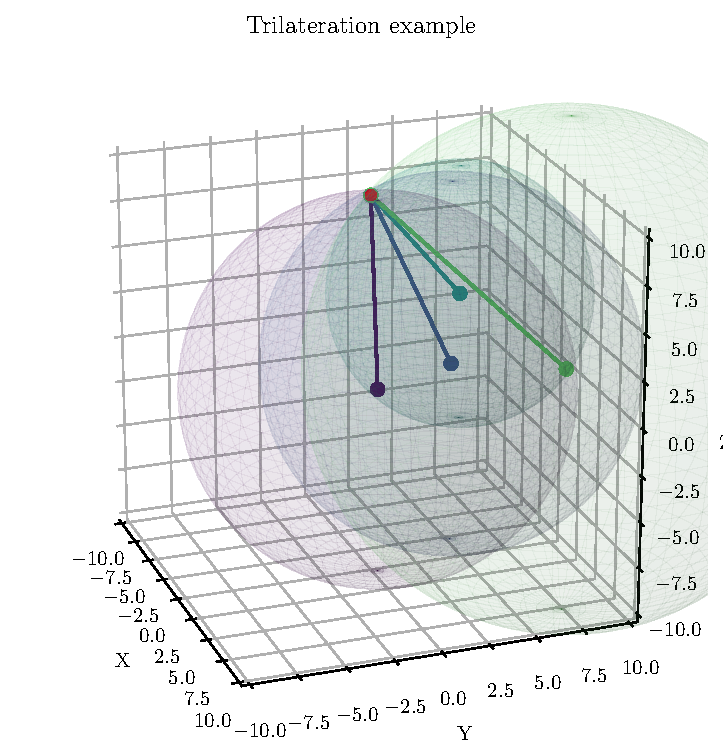
\includegraphics[width=0.4\textwidth]{figures/trilateration.pdf}
    \caption[Trilateration example.]{\textbf{Trilateration example.} 4 spheres detecting an unknown point in space, respecting the $n+1$ rule. The targeted point is found as the intersection of spheres, with no ambiguities.}
    \label{fig:trilateration}
\end{figure}


\subsection{Multidimensional Scaling algorithm}\label{sec:MDS}
MDS is a robust methods that allows to estimate points coordinates given the relative distances among them. Since it relies on fully-connected points, the algorithm results to be robust against noise, as one information, i.e. distance, is validated by another one. Indeed, given two generic points $X_i$ and $X_j$, the distance information $d_{i,\,j}$ obtained from the $i$-th point is supported by the distance $d_{j,\,i}$ read from the $j$-th point. In this way, the method is less dependent on the single piece of information that might be inaccurate, leading to a more balanced solution. Figure~\ref{fig:MDS_visualization} shows an example of fully-connected network of points, in which each node exchanges distance information with the others.\par

\begin{figure}[!ht]
    \centering
    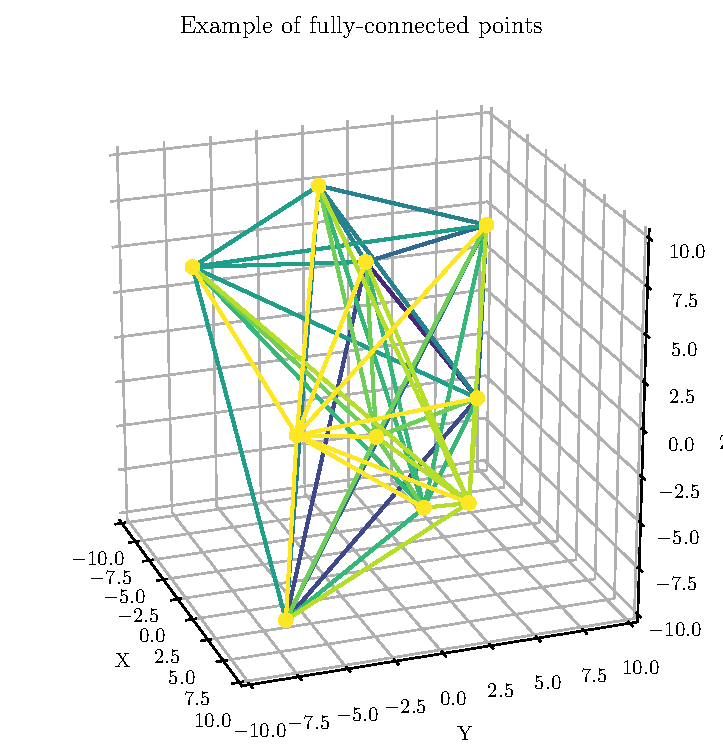
\includegraphics[width=0.4\textwidth]{figures/MDS_visualization.pdf}
    \caption[Example of fully-connected network.]{\textbf{Example of fully-connected network.} Each point communicates with the others, exchanging distance information. The Latin Hypecube Sampling was used for maximizing the distribution of points for this representation. The represented scenario is the input for the MDS algorithm.}
    \label{fig:MDS_visualization}
\end{figure}

The algorithm can be exploited for several applications, but a natural application lies in the estimation of the location of points in space. Specifically, it uses a square matrix of squared distances to build a relative map that describes the distribution of points in space  \cite{Li2021CooperativeNodes}. An example of distance matrix is reported in Equation~\ref{eq:distance_matrix_example}. In details, $d_{i,\,j}$ represents the squared distance between point $i$ and point $j$. Naturally, $d_{j,\,i}$ represents the squared distance between point $j$ and point $i$. In an error- and noise-free scenario, $d_{i,\,j} = d_{j,\,i}$ whilst in a real-case application the two elements might differ due to background noise, latency or interference. \par

\begin{equation}
    \label{eq:distance_matrix_example}
    D = 
    \begin{bmatrix}
    d_{1,1} & d_{1,2} & \dots & d_{1,N} \\
    d_{2,1} & d_{2,2} & \dots & d_{2,N} \\
    \vdots & \vdots & \ddots &  \vdots & \\
    d_{N,1} & d_{N,2} & \dots & d_{N,N} \\
    \end{bmatrix}
\end{equation}

The algorithm results to be easy and flexible and can be summarized in two major steps: \textit{1)} estimation of a relative map from the distance matrix and \textit{2)} transformation of the relative map in the absolute one. The following paragraphs better describe the two steps.\par

\subsubsection{From distance matrix to relative map}\label{sec:from_d_to_rel_map}
The core of MDS relies on the eigendecomposition of a symmetric matrix $D$ of square distances to estimate the relative map of the involved points. \par

Given the $D$ matrix, it is possible to write the associated eigendecomposition by introducing the centering operator $\textbf{H} = \textbf{I} - \textbf{ee}^T/N$, with $N$ dimension of the matrix. The new centered matrix is reported in the left-hand side of Equation~\ref{eq:eigendecomposition}, while the associated decomposition on its right-hand side.

\begin{equation}
    \label{eq:eigendecomposition}
    -\frac{1}{2}\textbf{H}\textbf{D}\textbf{H} = \textbf{U} \boldsymbol{\Lambda}\textbf{U}^T
\end{equation}

Eventually, the relative map $\Tilde{X}$ can be estimated by computing

\begin{equation}
    \Tilde{X} = \boldsymbol{\Lambda}^\frac{1}{2}\textbf{U}^T
\end{equation}

The relative map is a map that describes the location of points in space. It might be affected by unknown Cartesian transformation such as translation, rotation and flip. The fact that a relative configuration can correspond to multiple absolute ones has been called in the literature ambiguity.

\subsubsection{From relative to global map}
In order to turn a relative map to a global map, i.e. the correct estimation of the involved nodes, the ambiguities introduced in Section~\ref{sec:from_d_to_rel_map} must be completely solved. 
In order to achieve that, at least $n+1$ points with known location have to be used. \par

Several methods are known in the literature to solve such problem. Most of them are explained in details in \cite{RisteskaStojkoska2014NodesAlgorithm}. However, thanks to its reliability and accuracy, the Singular Value Decomposition (SVD) method has been chosen for this application, and the following paragraph will explain it in details. \par

Let $p = \left[p_1, p_2, \dots, p_{n+1}\right]$ and $q = \left[q_1, q_2, \dots, q_{n+1}\right]$ two sets of corresponding anchors, where $q$ represents the set of true coordinates and $p$ the estimated one coming out from the eigendecomposition step.

\begin{enumerate}
    \item Compute the weighted centroids of both point sets
    \begin{equation}
        \Bar{p} = \frac{1}{n+1} \sum_{i=1}^{n+1} p_i \text{,}\quad \Bar{q} = \frac{1}{n+1} \sum_{i=1}^{n+1} q_i
    \end{equation}

    \item Compute the centered vectors
    \begin{equation}
        p_i' = p_i - \Bar{p} \text{,}\quad q_i' = q_i - \Bar{q}\text{,}  \quad \forall i \in \left[1, n+1\right]
    \end{equation}

    \item Compute the $n\times n$ covariance matrix
    \begin{equation}
        C =  P' {Q'}^T
    \end{equation}
    where $P'$ and $Q'$ are the $n \times (n+1)$ matrices that have $p_i'$ and $q_i'$ as their columns, respectively.

    \item Compute the singular value decomposition
    \begin{equation}
        C = U\Sigma V^T
    \end{equation}
\end{enumerate}

The unknown rotation can be obtained as
\begin{equation}
    R = V U^T
\end{equation}

while the unknown translation as
\begin{equation}
    t = \Bar{q} - R\Bar{p}
\end{equation}

Therefore, the global map can be written as
\begin{equation}
    \hat{X} = R \Tilde{X} + t
\end{equation}

Please note that with the SVD method, no flip ambiguities must be solved.

% \begin{algorithm}
%     \caption{Multi-Dimensional Scaling algorithm}\label{alg:MDS}
%     \begin{algorithmic}
%     \State{\textbf{Result:} Estimated location of nodes}
%     \State{Initialization}

%     \State Read distances and send information over the network
%     \State Assemble the distance matrix
%     \State Center the matrix
%     \State Compute relative map via Eigendecomposition
%     \end{algorithmic}
% \end{algorithm}



% Methodology
% DA RISCRIVERE DISTRIBUENDO IL CONTENUTO NEI VARI ALTRI BULLET POINTS DI QUESTA SEZIONE
% Our scenario has a swarm in which one of the drones acts as an anchor.
% The anchor is allowed to move independently and faster, while keep moving in the same direction of the swarm.
% The objective is to move collect the measurement in four points relatively to the reference frame in which we consider the swarm, to collect the data required by the algorithm (WLP and MDS)
% The algorithms have been tested in two type of simulated environments: 
% The first with a node simulating the dynamic of the drones, capable of managing more than 10 drones and which allows us to perform our studies.
% The second with Gazebo+Ardupilot, for performing a simulation with the SITL and getting closer to a real application of the algorithm on physical robots. Unfortunately, this version is computational-heavy and we were able to run the simulation with XX drones at the most.
% In both cases, the operating entities were executing in a ROS 2 project object of our work.
% Sottolineare che abbiamo la simulazione con test e la simulazione con Gazebo. ABbiamo fatto test perchè più veloce.
% Activity diagram per spiegare i passaggi, quasi impostato come macchina a stati finiti.
% Dire che abbiamo usato ROS 2, foto dei topic sia stilizzata che completa in appendice con 10 droni
% Foto Gazebo con il mondo con i dron


\section{Methodology}\label{sec:methodology_section}
This section describes the main aspects of the implementation not yet adequately depicted and the methodologies employed to verify the performances of the discussed techniques.
The implementation consists of a ROS 2 project where the goal is to estimate the position of the drones in a swarm using the measurements of their relative distances. The swarm operates in a simulated environment, which can be of two types. In the first type, a dedicated ROS 2 node is responsible for simulating the drones dynamics solely via numerical integration, while the second adopts the physical simulator Gazebo\footnote{https://gazebosim.org/home}. 
To make this second simulation even more realistic, the commands are routed through ArduCopter\footnote{https://ardupilot.org/copter/} via Mavros\footnote{https://github.com/mavlink/mavros}.

The reason why two simulation types were developed is twofold. First, in this way the project is more modular and scalable. Second, running a simulation with Gazebo and a Mavros node for each drone is computational heavy and no adequate computational resources were available for this purpose. Still, the Gazebo+Ardupilot combination serves the purpose of closely simulating the Software-In-The-Loop (SITL) environment, bridging the gap towards real-world deployment.
Figure~\ref{fig:gazebo_setup} illustrates the Gazebo setup in the case of 3 drones.

\begin{figure}[!ht]
  \begin{center}    
    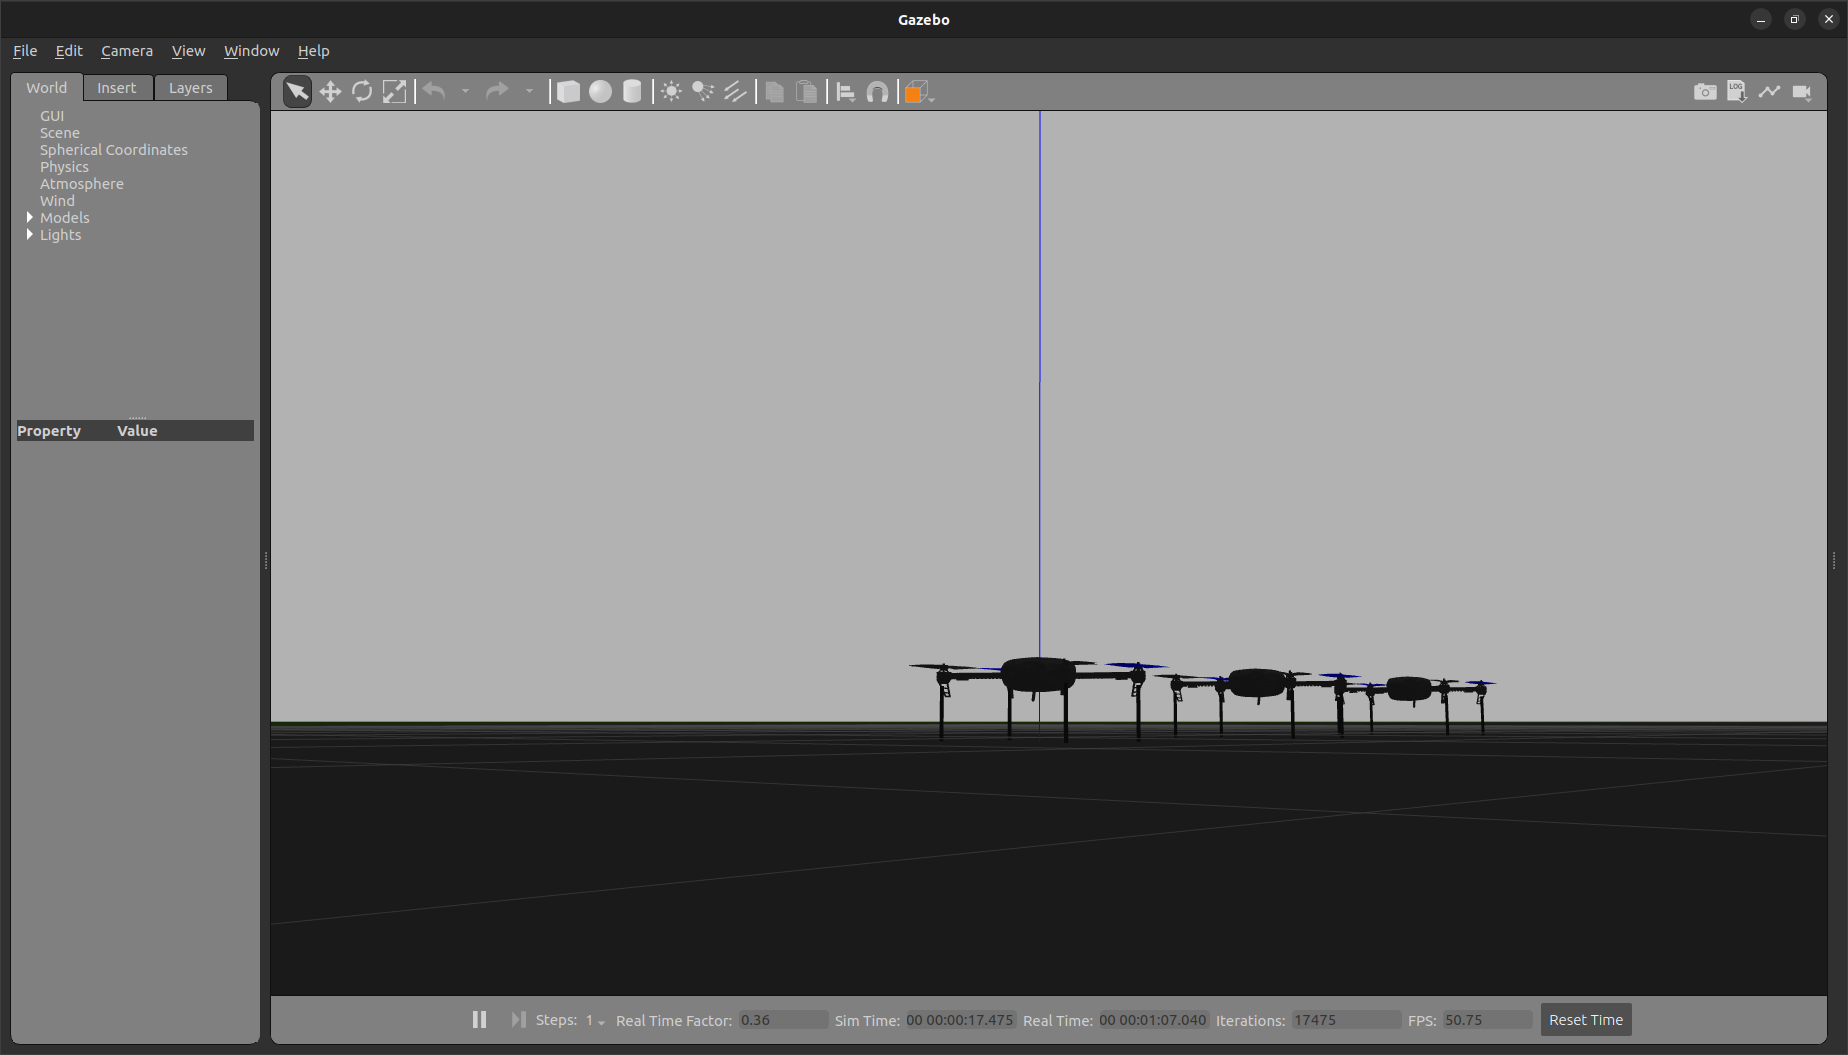
\includegraphics[width=0.45\textwidth]{figures/gazebo-environment.png}
  \end{center}
  \caption[Gazebo setup]{
    \textbf{Gazebo setup.} 
    Gazebo simulator and runway world for simulating the guidance of a swarm of drones while estimating their positions.
  }
  \label{fig:gazebo_setup}
\end{figure}

In the following, the process regarding the data collection for such scenario will be better explained. Subsequently, the blocks composing the ROS 2 project will be better illustrated, highlighting how they interact, both in the case of simple numerical simulator and with Gazebo. Finally, the experiment procedure will be exposed and explained, leading to the comparison of the two algorithms, i.e. trilateration and MDS.



\subsection{Infrastructure-free localization}
In this section, the approach for an infrastructure-free localization of drones is presented, operating within a WSN. 
Unlike traditional methods that rely on a fixed set of anchor nodes to determine drone locations, this research embraces a novel approach inspired by recent trends in the literature. This approach involves designating a single drone within the swarm as the “anchor node”, which moves faster than the others and is in charge of collecting distance measurements from various points.
As reiterated multiple times, both of the compared algorithms are only able to solve the problem if equipped with 4 sets of measurements from distinct points. 

In the project, the reference system with respect to which the positions of the drones are calculated is centered at the position of the anchor. In both the simulation types, the drone designated as the anchor is the one called \textit{drone1}. In the case of the numerical simulation, its initial position is $x_0^1=[0.0,0.0,5.0]^\top$\footnote{In the notation, subscript refers to time, and superscript to drone.}, while in Gazebo it is in at the origin of the absolute reference frame. 
In contrast, the position of the other drones is randomly generated in all coordinates. \par

During the simulation, the swarm is moved at a constant speed in a predefined direction. 
The anchor drone is subject to the same movement of the swarm, but, in addition to it, it also continuously changes its position to collect new measurements from different points.
This is achieved by imposing to the anchor not only the swarm velocity, but also an additional one depending on the direction it has to follow. \par

Once the anchor has moved in a certain direction for a given time (which can be affected by noise), it remains still relatively to the swarm, to complete the distances collection and perform an estimation of the swarm configuration through the localization algorithms.
After this, a new direction is assigned to the anchor and the cycle is repeated. Figure~\ref{fig:flowchart} presents a flowchart with the main steps of the described approach, while Figure~\ref{fig:sequence} the screenshots obtained by executing the project with no noise for an anchor movement.

\begin{figure}[!ht]
  \begin{center}
    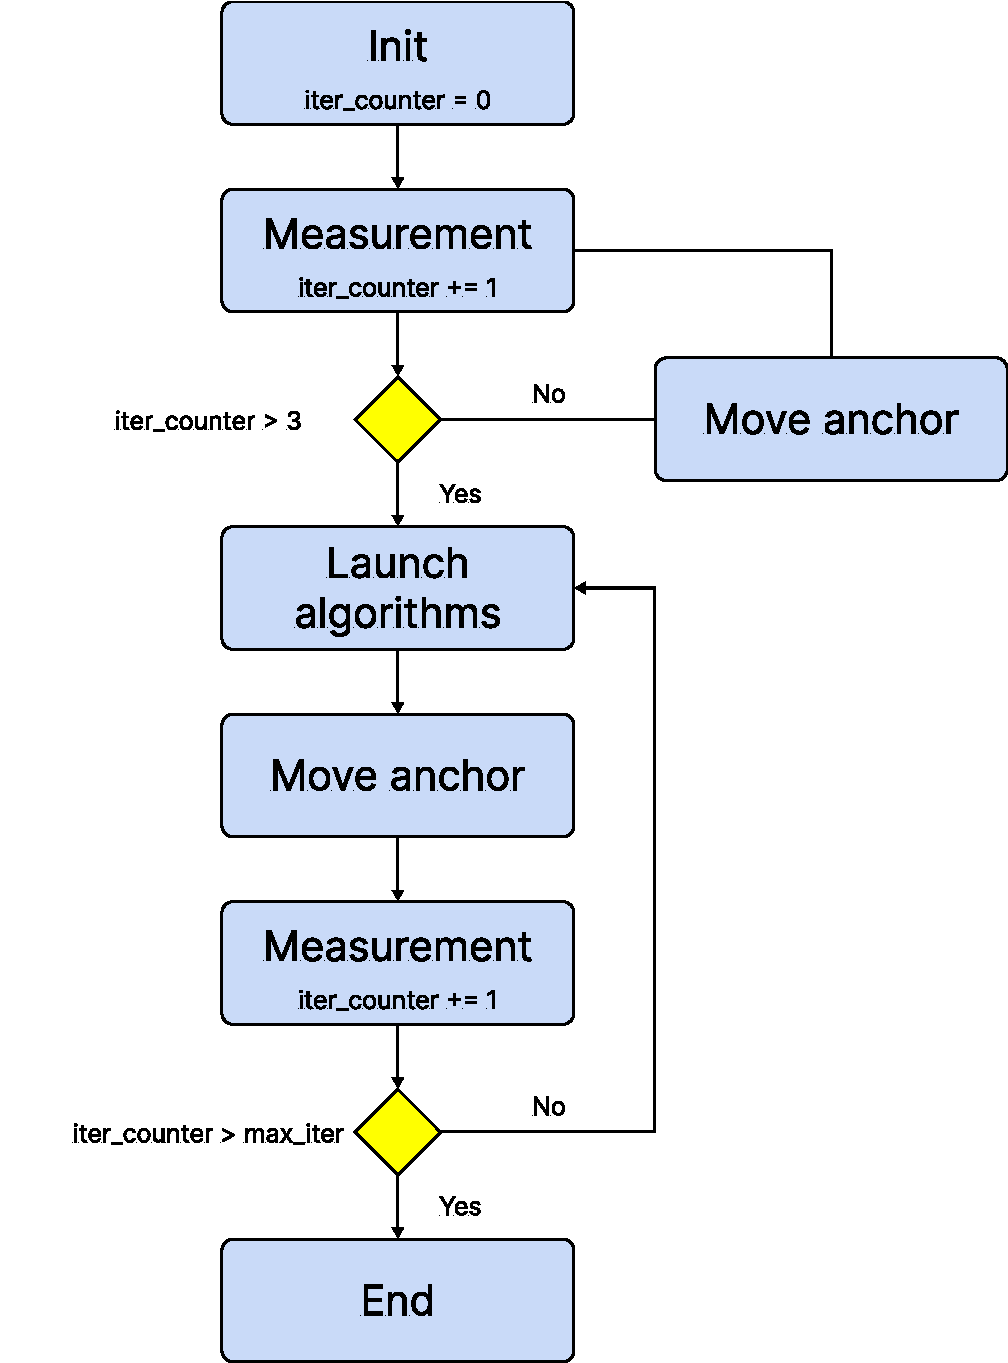
\includegraphics[width=0.37\textwidth]{figures/flowchart_color.pdf}
  \end{center}
  \caption[Software flowchart]{
    \textbf{Software flowchart.} 
    The diagram illustrates the main steps of the implemented approach. This was used for both the simulation types. The first loop is necessary to make sure to have at least four sets of measurements. The second cycle, on the other hand, is the one continuously performed to estimate the drones position.
  }
  \label{fig:flowchart}
\end{figure}


\begin{figure*}[!ht]
     \centering
     \begin{subfigure}[b]{0.28\textwidth}
         \centering
         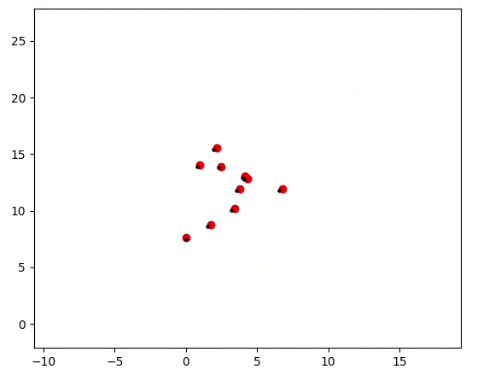
\includegraphics[width=\textwidth]{figures/sequence_1.png}
         \caption{Step 1.}
         \label{fig:sequence_1}
     \end{subfigure}
     \hfill
     \begin{subfigure}[b]{0.28\textwidth}
         \centering
         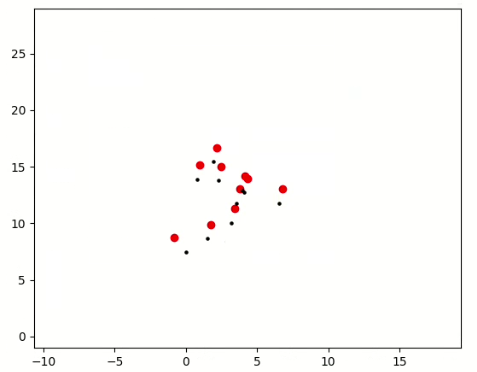
\includegraphics[width=\textwidth]{figures/sequence_2.png}
         \caption{Step 2.}
         \label{fig:sequence_2}
     \end{subfigure}
     \hfill%
      \begin{subfigure}[b]{0.28\textwidth}
         \centering
         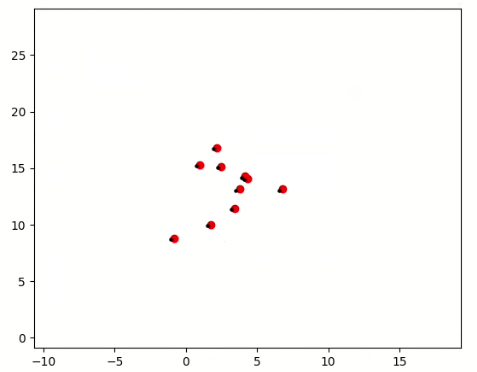
\includegraphics[width=\textwidth]{figures/sequence_3.png}
         \caption{Step 3.}
         \label{fig:sequence_3}
     \end{subfigure}
     \hfill
     \caption[Algorithm iteration]{
        \textbf{Algorithm iteration.} 
        This screenshots illustrate the main steps of an iteration of the algorithm. The anchor starts moving from a point in which the data collection and estimation have been performed (\ref{fig:sequence_1}). While moving, the rest of the swarm moves toward a predefined direction, positive $y$ in the case shown (\ref{fig:sequence_2}). After a given time, the anchor stops and remains in the same relative position for a new data collection and estimation, until the next iteration (\ref{fig:sequence_3}). 
      }
     \label{fig:sequence}
\end{figure*}


\subsection{Architecture}
The project is built upon ROS 2, with key nodes designed to fulfill specific roles within the system architecture.
The core node is the one called \textit{main}, which is responsible for guiding drones, reading distance measurements, running algorithms and tracking results. 
Another important node, called \textit{hub}, reads the coordinates from the environment (either the numerical simulator or Gazebo) and returns the distances, possibly adding noise. This functionality simulates the adoption of real UWB sensors. 

The numerical simulator node (i.e. \textit{test}) is responsible for tracking drones' positions, simulating the application of velocity commands, and incorporating dynamic model noise to represent real-world motion behaviors.
Other nodes were adopted when using Gazebo: the Mavros nodes, for communicating between the scripts, and the Ardupilot plugin.

The simplified diagram in Figure~\ref{fig:nodes_architecture} provides a visual representation of the simulation setup, highlighting the main nodes and topics\footnote{In ROS 2, a topic is a named channel of communication that facilitates the exchange of data between different nodes.}. 
The diagram resembles the one obtained by launching the rqt\_graph\footnote{http://wiki.ros.org/rqt\_graph} tool. For clarity, only the connections of 3 drones are illustrated.

% The diagram resembles the one obtained launching the rqt\_graph \footnote{http://wiki.ros.org/rqt_graph} tool, but, for clarity, only 3 drones are considered in the diagram, but when using the numerical simulator more nodes can be managed. On the other hand, when using Gazebo, we were able to run the simulation with three drones at the most. % Appendix A provides the diagram obtained running the rqt\_graph\footnote{http://wiki.ros.org/rqt_graph} tool when Gazebo is operating.

\begin{figure}[!ht]
  \begin{center}
    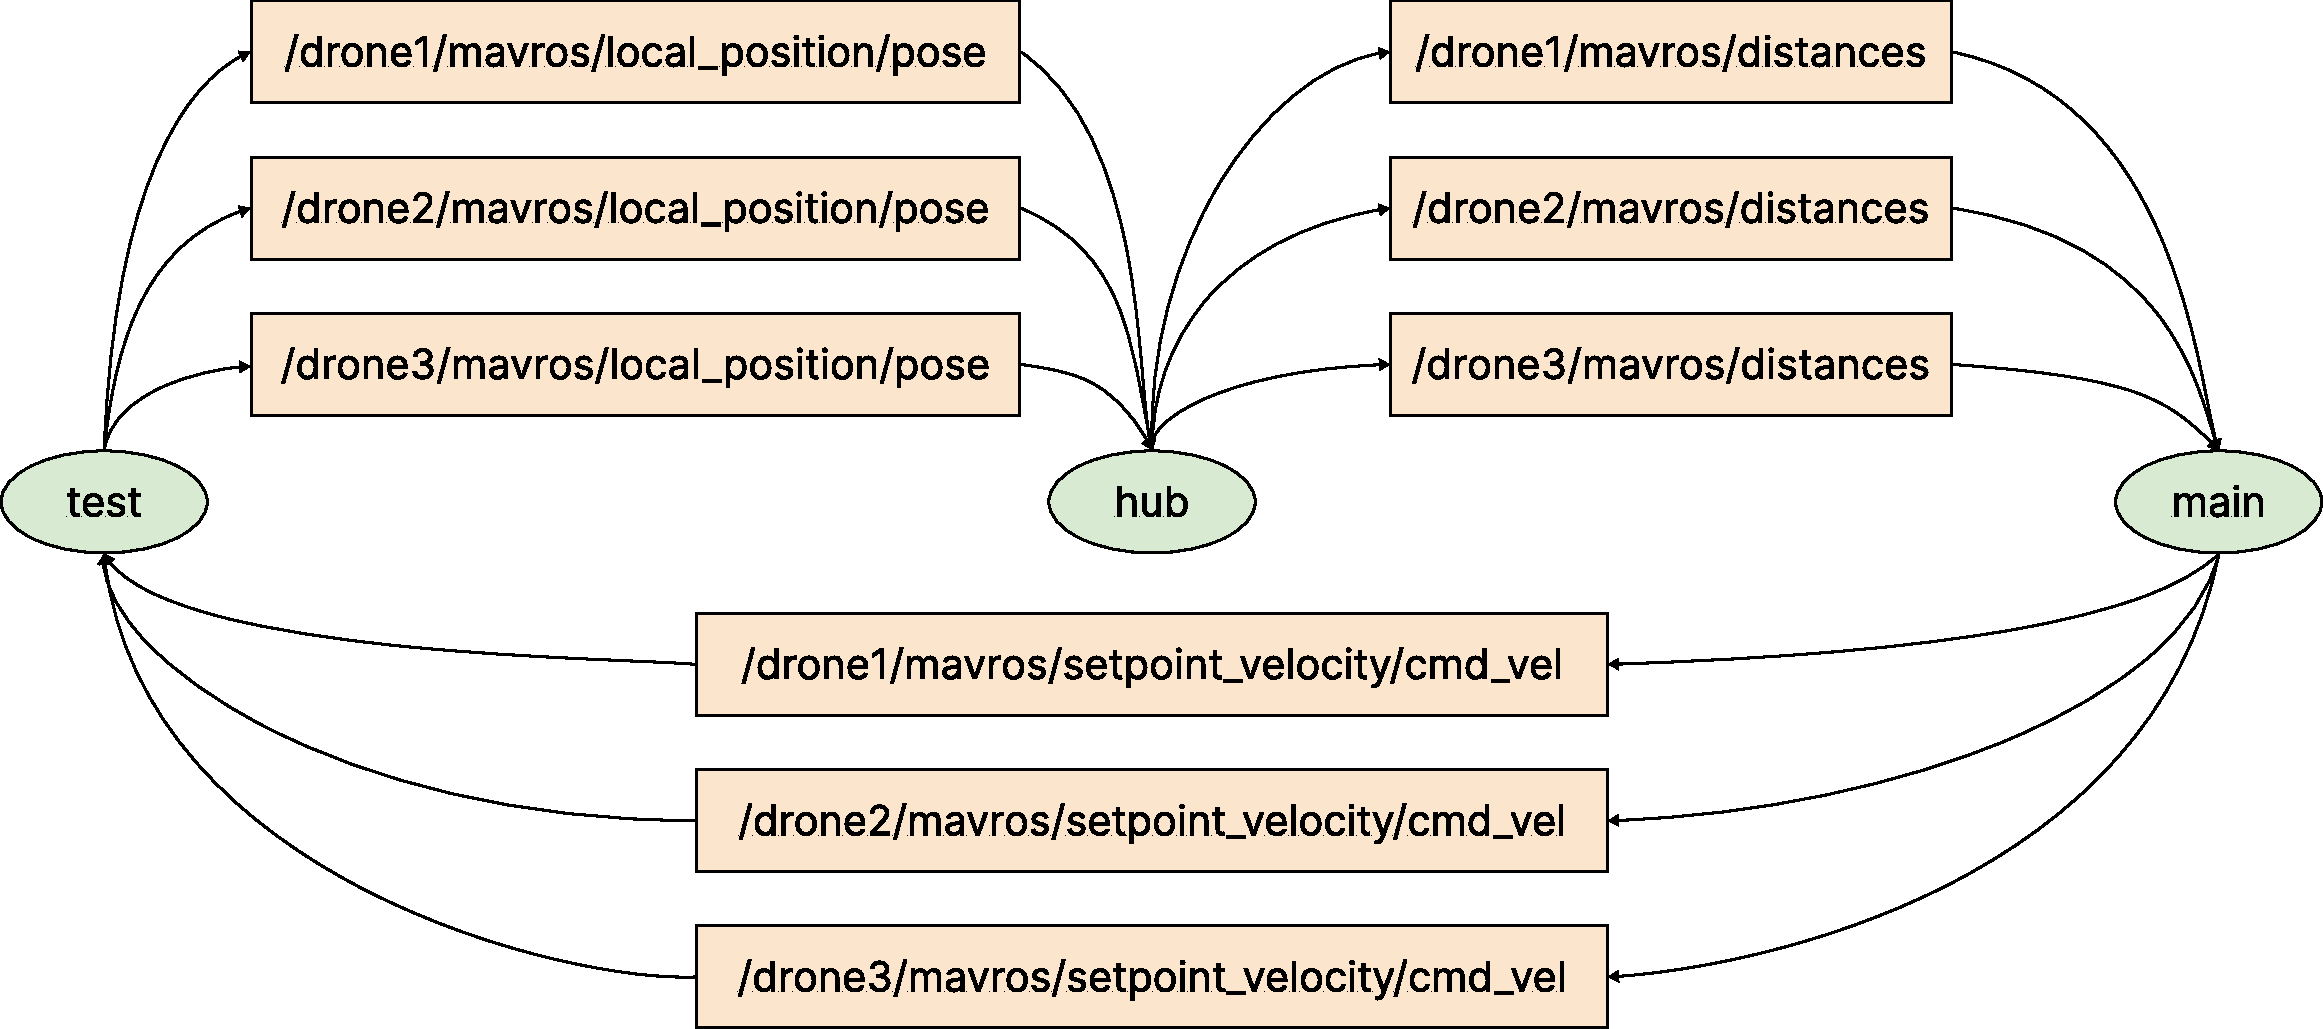
\includegraphics[width=0.47\textwidth]{figures/nodes_architecture_color.pdf}
  \end{center}
  \caption[Nodes architecture]{
    \textbf{Nodes architecture.} 
    Graph showing the connections between the main nodes operating when running the project for 3 drones with the numerical simulator. Each node is represented with an ellipse, while the topics are in rectangles. The graph has bee redrawn from that obtained using the rqt\_graph tool. Some of the connections needed in the real implementation have been deleted for clarity.
  }
  \label{fig:nodes_architecture}
\end{figure}

\subsection{Experimental setup}
To evaluate the performance of the two algorithms, a series of targeted experiments was carried out, mostly using the numerical simulator. 
This approach enabled to run multiple experiments with different settings and aggregate performance metrics for robust conclusions. 
These experiments encompassed distinct settings, each characterized by specific noises. The types of noise considered are: $a)$ the noise affecting the distance measurement, which is set by the hub; $b)$ the noise that affects the time for which a node continues to move along a specific direction, compromising the accurate knowledge of the anchor position; $c)$ a noise affecting the system dynamics.\par

All the noises are assumed to come from Gaussian distributions centered in zero and with a standard deviation specified via parameters.\par

The algorithms were assessed across five distinct settings: no noise, one noise out of three per time, and all three present together. Table~\ref{tab:std_summary_comparison} summarizes the standard deviations characterizing the different noises for the tested setting. 
\begin{table}[!ht]
    \centering
    \begin{tabular}{l|ccccc}
      \textbf{Quantity} & 
      \textbf{setting1} &
      \textbf{setting2} &
      \textbf{setting3} &
      \textbf{setting4} & 
      \textbf{setting5} \\
      \hline
      Distance [m]& 0.0 & 0.05 & 0.0   & 0.0 & 0.05   \\
      Time [s] & 0.0 & 0.0  & 0.0   & 0.2 & 0.2    \\
      Dynamics [m]& 0.0 & 0.0  & 0.001 & 0.0 & 0.001  \\
    \end{tabular}
      \caption[Setting details]{
        \textbf{Setting details.}
        The standard deviations of the Gaussian-distributed, zero-mean noises affecting the considered quantities is reported for the different tested settings.
    }
    \label{tab:std_summary_comparison}
\end{table}


Each setting underwent 50 runs with 33 anchor movements and 30 algorithm executions (i.e. 30 iterations of the second cycle in the diagram in Figure~\ref{fig:flowchart} started after having collected 3 set of measurement). Each time the project is executed, the number of drones can be specified by a parameter. For data collection, the control of 10 drones was simulated, whose location is randomly generated using the number of runs being tested as a seed\footnote{In the context of a random number generator (RNG), a seed is an initial value that is used to start the generation process. It serves as the starting point for producing a sequence of seemingly random numbers.}, so that the comparison between different settings is fair. In addition, to facilitate the comparison and make it more meaningful, average errors are calculated by grouping both by setting and drone, as shown in the following section.


% Results
% Results
% Paragone sulla singola esecuzione fino a un tot di metri, 
% Screenshot multipli di un ciclo di ancora completo, a far vedere come:
% SI parte con una stima e ancora in 0,0,0
% Ogni volta che l’ancora fa un movimento MDS viene ricalcolato e la posizione ristabilita
% Le ellissi diventano via via più grandi
% Paragone su run multiple con noise

\section{Results}\label{sec:results_section}
This section presents the outcomes obtained through the implementation and execution of the trilateration and MDS algorithms for estimating the positions of drones in the scenarios and with the settings previously presented.\par

Table~\ref{tab:comparison} summarizes the main focus of this study: a comparative evaluation of the estimation errors achieved by employing the two algorithms. As expected, these findings affirm the superiority of MDS in terms of average estimation errors. \par

To compute the average performances, point-wise errors were calculated for each drone at every timestep, and grouped the results by settings. This categorization provides insights to the consistent outperformance of MDS over trilateration, regardless of the nature of the simulated noise impacting the execution.

\begin{table}[!ht]
  \centering
    \begin{tabular}{l|ccccc}
      \textbf{Algorithm} & 
      \textbf{setting1} &
      \textbf{setting2} &
      \textbf{setting3} &
      \textbf{setting4} & 
      \textbf{setting5} \\
      \hline
      MDS & 0.21 & 0.31 & 0.25 & 0.55 & 0.57 \\
      Trilateration & 0.35 & 0.41 & 0.34 & 0.83 & 0.86 \\
    \end{tabular}
    \caption[Average estimation errors by tested settings]{
        \textbf{Average estimation errors by tested settings.}
    }
    \label{tab:comparison}
\end{table}


Another result regards the value of the average estimation error. For each drone,it continuously increases iteration by iteration. \par

This trend, observable in Figure~\ref{fig:simulation_performances}, can be attributed to the influence of the drift, which is mostly caused by the action of the noises on the system. Additionally, it can be also related to the discrete-time nature of these computations, and it might be influenced by the timestep used for executing the project nodes.

\begin{figure*}[!ht]
     \centering
     \begin{subfigure}[b]{0.28\textwidth}
         \centering
         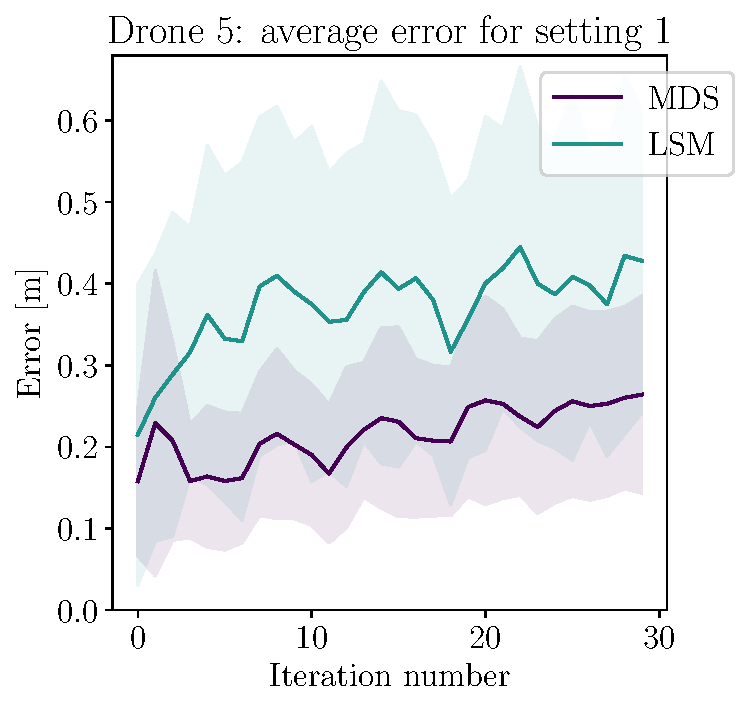
\includegraphics[width=\textwidth]{figures/drone5_setting1.pdf}
         \caption{Setting 1.}
         \label{fig:setting1_drone5}
     \end{subfigure}
     \hfill
     \begin{subfigure}[b]{0.28\textwidth}
         \centering
         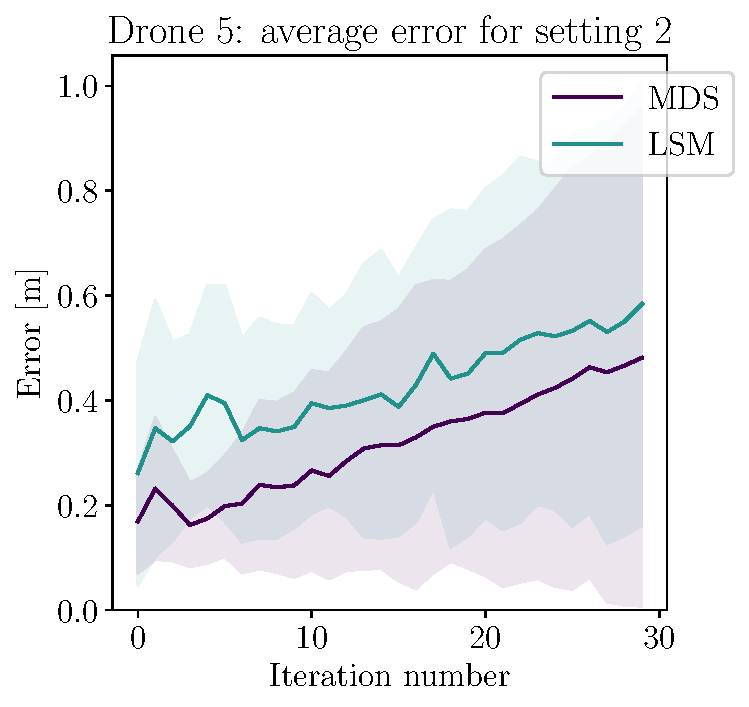
\includegraphics[width=\textwidth]{figures/drone5_setting2.pdf}
         \caption{Setting 2.}
         \label{fig:setting2_drone5}
     \end{subfigure}
     \hfill%
      \begin{subfigure}[b]{0.28\textwidth}
         \centering
         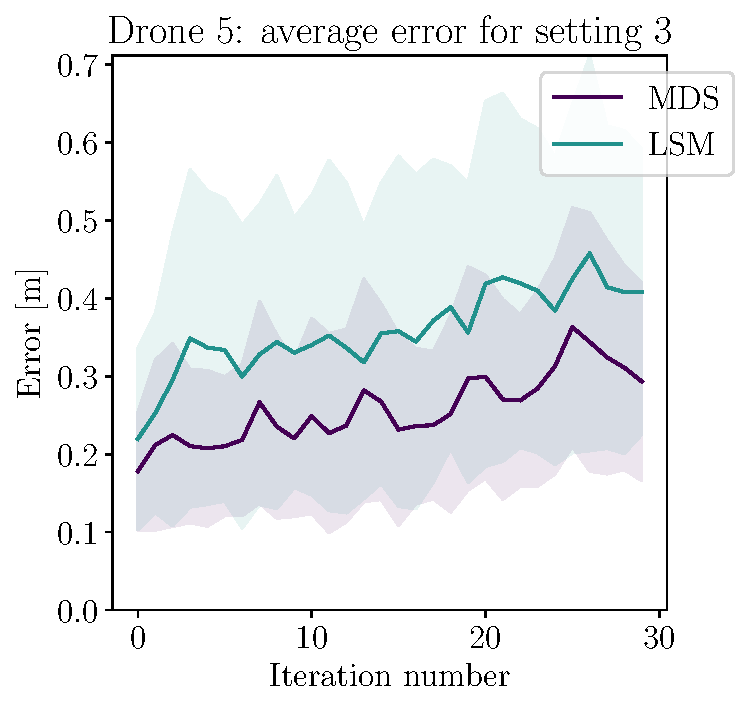
\includegraphics[width=\textwidth]{figures/drone5_setting3.pdf}
         \caption{Setting 3.}
         \label{fig:setting3_drone5}
     \end{subfigure}
     \hfill
     \begin{subfigure}[b]{0.28\textwidth}
         \centering
         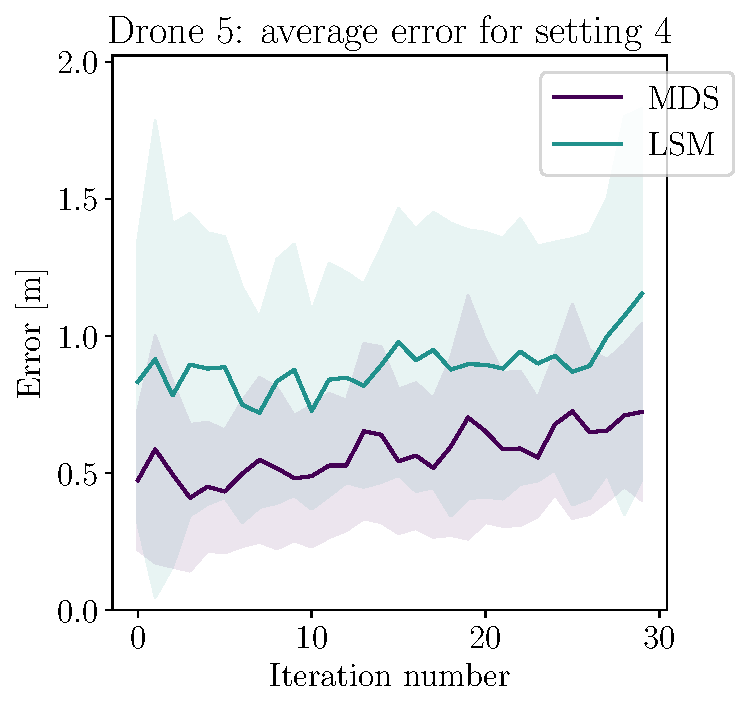
\includegraphics[width=\textwidth]{figures/drone5_setting4.pdf}
         \caption{Setting 4.}
         \label{fig:setting4_drone5}
     \end{subfigure}
     \hfill
     \begin{subfigure}[b]{0.28\textwidth}
         \centering
         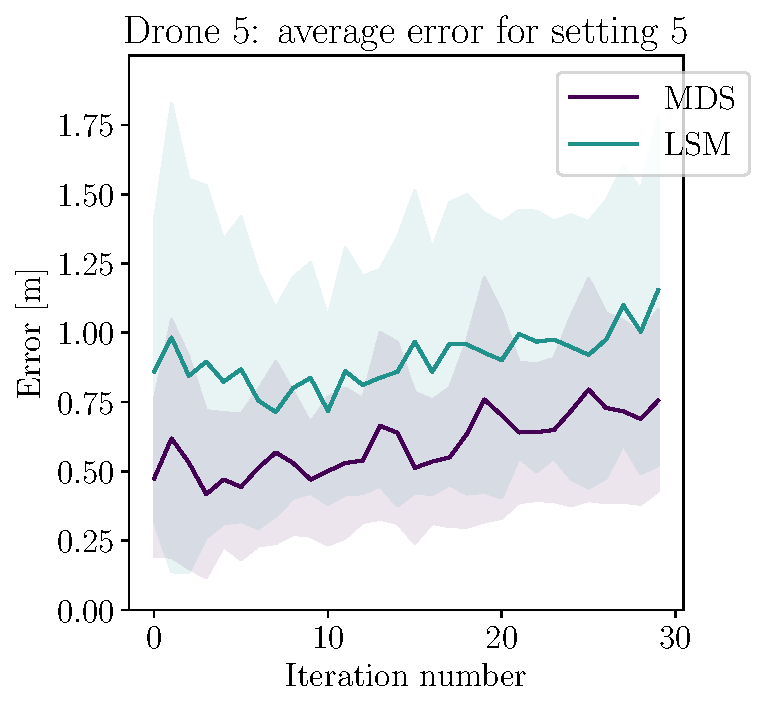
\includegraphics[width=\textwidth]{figures/drone5_setting5.pdf}
         \caption{Setting 5.}
         \label{fig:setting5_drone5}
     \end{subfigure}
     \hfill
     
     \caption[Drift]{
        \textbf{Drift.} 
        The five graphs illustrate the performances over time for the two considered algorithms. Specifically, the average estimation error and its trend for drone5 (chosen arbitrarily) is shown for the different tested settings. Independently, the average error always increases, highlighting the drift phenomenon. 
     }
     \label{fig:simulation_performances}
\end{figure*}

The comparison of different noises, based on the data collected, presents challenges due to varying attributes and quantity involved (e.g. distances, times, positions), but their effects are evident, especially for Setting 4 and Setting 5, observable respectively in Figure~\ref{fig:setting4_drone5} and Figure~\ref{fig:setting5_drone5}. \par

This outcome underlines the potential for enhancements in error mitigation strategies against noises and drifts, such as the introduction of global measurements or absolute re-calibration procedures, as elaborated in the last section. \par

% Finally, Figure~\ref{alg:MDS} offers a visual representation of this project's execution within the Gazebo environment. This portrayal highlights the project's competence in accurately estimating drone positions in real-time, particularly when operating within the Gazebo+Ardupilot framework. This environment closely mirrors real-world deployment conditions, further validating the potentiality of this work. \par

Table~\ref{tab:error_reduction} illustrates the great performances of MDS over trilateration. Indeed, the algorithm provided an error reduction between $24.4\%$ and $40.0\%$. A noticeable information is that an error reduction of about $33.7\%$ was achieved in Setting 5, namely the most noisy and complex scenario tested. This directly highlights the strong capabilities and reliability of MDS. \par           

However, few improvements could be introduced to obtain even higher results. First of all, different MDS versions could be integrated, to better overcome the different type of noise and reduce the computational times. Example of those are enhanced Multidimensional Scaling (eMDS) \cite{eMDS}, dynamic Multidimensional Scaling (dMDS) \cite{dMDS}, MDS-MAP or GM-MDS. \par

\begin{table}[!ht]
  \centering
    \begin{tabular}{l|c}
      \textbf{Configuration} & \textbf{Error reduction} \\\hline
      Setting1 & $40.0\%$ \\\hline
      Setting2 & $24.4\%$ \\\hline
      Setting3 & $26.5\%$ \\\hline
      Setting4 & $33.7\%$ \\\hline
      Setting5 & $33.7\%$ \\\hline
    \end{tabular}
    \caption[Average error reduction by relying on MDS algorithm]{
        \textbf{Average error reduction by relying on MDS algorithm}: in the table the reduction in the average error is shown, by relying on the MDS algorithm for drones coordinates estimation instead of standard trilateration algorithm.  
    }
    \label{tab:error_reduction}
\end{table}

Additionally, partially-connected swarms could be studied and implemented with the introduction of distributed MDS and distributed-weighted MDS (dwMDS), to better face the weakness or absence of intercommunication among the drones, due to the presence of obstacles. \par

Another interesting research is the integration of such simulation with Kalmann filters, to better estimate the position of drones via a measurement-update approach. In particular, the estimation of the covariance matrix associated to the location of each drone could be used to update more accurately the covariance in the filter, in order to take advantage of the best features of both the tools.

% Conclusion
\section{Conclusion}\label{sec:conclusion_section}
This paper illustrated the implementation of the Multidimensional Scaling algorithm and the performances that can be obtained when it is used for estimating the location of a swarm of drones. Particularly, two different simulations were assessed to demonstrate its potential: a numerical one to collect data and to compute the average behaviour and the associated error, and a Software-in-the-loop one to demonstrate potential real-world applications. \par

The performance metrics were compared to a more classical but less robust algorithms known in the literature as trilateration. It has demonstrated that MDS always outperformed trilateration in all the different studied scenarios, in which different Gaussian-distributed noise was added to dynamics, measurement or clock-time. \par

The method studied in this work introduces for the first time the estimation of a swarm of fully-connected drones via infrastructure-free measurements, in which one node, designated as anchor, is responsible to move around and collect different measurements to make the algorithm run. \par

Future improvements and further studies can be conducted, such as the introduction of an extended-MDS or the integration of its covariance estimation to better update a Kalmann filter.




% if have a single appendix:
%\appendix[Proof of the Zonklar Equations]
% or
%\appendix  % for no appendix heading
% do not use \section anymore after \appendix, only \section*
% is possibly needed

% use appendices with more than one appendix
% then use \section to start each appendix
% you must declare a \section before using any
% \subsection or using \label (\appendices by itself
% starts a section numbered zero.)
%


% \appendices
% \section{Proof of the First Zonklar Equation}
% Appendix one text goes here.

% % you can choose not to have a title for an appendix
% % if you want by leaving the argument blank
% \section{}
% Appendix two text goes here.


% % use section* for acknowledgment
% \section*{Acknowledgment}


% The authors would like to thank...


% Can use something like this to put references on a page
% by themselves when using endfloat and the captionsoff option.
\ifCLASSOPTIONcaptionsoff
  \newpage
\fi



% trigger a \newpage just before the given reference
% number - used to balance the columns on the last page
% adjust value as needed - may need to be readjusted if
% the document is modified later
%\IEEEtriggeratref{8}
% The "triggered" command can be changed if desired:
%\IEEEtriggercmd{\enlargethispage{-5in}}

% references section

% can use a bibliography generated by BibTeX as a .bbl file
% BibTeX documentation can be easily obtained at:
% http://mirror.ctan.org/biblio/bibtex/contrib/doc/
% The IEEEtran BibTeX style support page is at:
% http://www.michaelshell.org/tex/ieeetran/bibtex/
%\bibliographystyle{IEEEtran}
% argument is your BibTeX string definitions and bibliography database(s)
%\bibliography{IEEEabrv,../bib/paper}
%
% <OR> manually copy in the resultant .bbl file
% set second argument of \begin to the number of references
% % (used to reserve space for the reference number labels box)
% \begin{thebibliography}{1}

% \bibitem{IEEEhowto:kopka}
% H.~Kopka and P.~W. Daly, \emph{A Guide to \LaTeX}, 3rd~ed.\hskip 1em plus
%   0.5em minus 0.4em\relax Harlow, England: Addison-Wesley, 1999.

% \end{thebibliography}

\bibliographystyle{./IEEEtran}
% \bibliography{references}
\bibliography{references}

\end{document}


 